\section{Logistic Regression}
\smallskip \hrule height 2pt \smallskip

Another probabilistic approach to classification (categorical predictions).  
 \hfill \\
Discriminative: learn $P(Y|X)$ directly then discriminate between classes.    % Week 5 audio. 
We solved similar problems using Bayes before (a generative approach).  
	But if we don't want to bother with modeling all those joint or conditional probabilities, we can do this discriminative approach instead. \hfill \\  %Wed 2/3 audio transcription.

Logistic Regression is the discriminative counterpart to a Naive Bayes generative classifier over Boolean features.  % https://www.cs.cmu.edu/~tom/mlbook/NBayesLogReg.pdf
The difference between logistic and Naive Bayes is just one word: "conditional".   % wk 5 audio
We are maximizing conditional log likelihood, that is conditional on X.  
	We are not going to spend our time encoding the distribution over X.   % wk 5 audio

\hfill \\   \hfill \\

Can use discrete or continuous outputs. \hfill \\ % https://www.youtube.com/watch?v=zAULhNrnuL4
It's a linear classifier; the decision rule is a hyperplane. \hfill \\  % Slide 6 summary
You optimize it (find weights) by gradient ascent, which works because it is concave.    \hfill \\  % Slide 6 summary
You can use "maximum conditional a posteriori" for regularization.    \hfill \\  % Slide 6 summary

\hfill \\ 

\underline{Summary from non-class sources:} \hfill \\
% https://www.youtube.com/watch?v=-Z2a_mzl9LM
We are still using linear regression in the inputs, but putting the result into a sigmoid function. \hfill \\
Recall $w_0 + w_1 x_1 + w_2 x_2 + w_3 x_3 = w^Tx$ and $x = (1, x_1, x_2, x_3)$.  \hfill \\
$P(death|x) = \sigma(w^Tx)$  %https://www.youtube.com/watch?v=-Z2a_mzl9LM
where $\sigma$, the sigmoid function,  converts your regression output into a sigmoid curve. \hfill \\
$\displaystyle \sigma(a) = \frac{1}{1+ e^{-a}} = \frac{1}{1+ e^{-(w_0 + w_1 x_1 + w_2 x_2 + w_3 x_3)}} = \frac{1}{1+ e^{-(w^Tx)}}$   \hfill \\ % https://www.youtube.com/watch?v=-Z2a_mzl9LM
\hfill \\

% https://www.youtube.com/watch?v=_Po-xZJflPM  :
We can convert this to a linear relationship by "taking the logit". \hfill \\
The logit (log odds) is the inverse of the logistic.  \hfill \\ %  https://en.wikipedia.org/wiki/Logistic_regression
$F(x) = \sigma(a)$ above.  It is the probability that the dependent variable equals a case, given some linear combination of the predictors.  It can range from $- \infty$ to $\infty$   % https://en.wikipedia.org/wiki/Logistic_regression
The logit is $\ln \frac{F(x)}{1-F(x)}$, or equivalently, after exponentiating both sides: \hfill \\
$\frac{F(x)}{1-F(x)} = e^{w^Tx}$  \hfill \\
The logit (i.e., log-odds or natural logarithm of the odds) is equivalent to the linear regression expression.

 


Note used odds ratio: $\frac{p}{1-p}$  \hfill \\
$\logit(\frac{1}{1+ e^{-(w^Tx)}}) = \log(\frac{\frac{1}{1+ e^{-(w^Tx)}}}{1-\frac{1}{1+ e^{-(w^Tx)}}}) $  \hfill \\ % https://www.youtube.com/watch?v=_Po-xZJflPM
We can now proceed with linear regression.  \hfill \\
Note that our predictions are now on the log scale; this impacts interpretation of the coefficients.  \hfill \\  %https://www.youtube.com/watch?v=_Po-xZJflPM 

\hfill \\ \hfill \\   

\underline{Lecture's presentation:} \hfill \\

Notation:  \hfill \\
\begin{itemize}
	\item $x_i^j$: the $i^{th}$ attribute of data point $j$
	\item $y^j$: the $j^{th}$ class  %(?)
	\item $x^j$: the $j^{th}$ training example
\end{itemize}

Once again we don't want to try to estimate $P(X,Y)$; that is challenging due to the size of the distribution. \hfill \\
We could make the Naive Bayes assumption and only need to calculate $P(X_i | Y)$, 
but if we want $P(Y|X)$, why not learn that directly?  You can use logistic regression. 
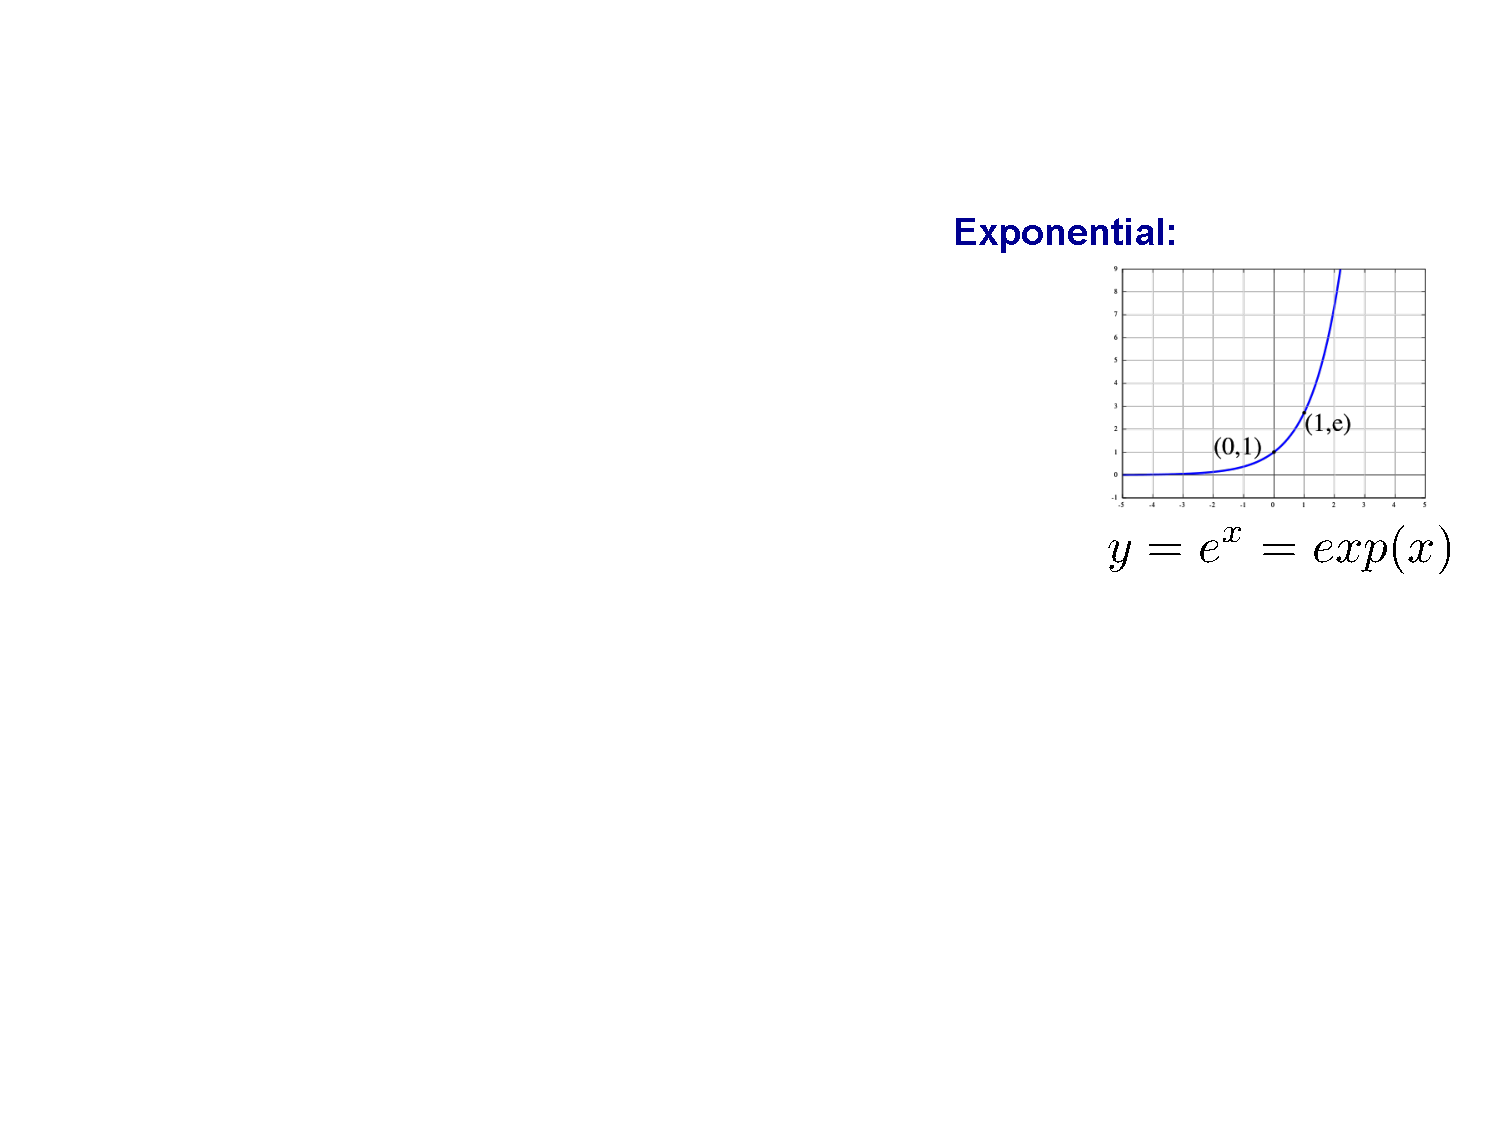
\includegraphics[width=1.5in]{figures/expo.pdf}     \hfill \\
\hfill \\

Reuse ideas from regression, but let the y-intercept define the probability.  \hfill \\
$P(Y=1|\bm{X, w}) \propto exp(w_0 + \sum_i w_i X_i)$  \hfill \\
With normalization constants:  \hfill \\
$\displaystyle  P(Y=0|\bm{X, w}) \frac{1}{1+ exp(w_0 + \sum_i w_i X_i)} $ \hfill \\
$\displaystyle  P(Y=1|\bm{X, w}) \frac{exp(w_0 + \sum_i w_i X_i)}{1+ exp(w_0 + \sum_i w_i X_i)} $ \hfill \\
Logistic function: 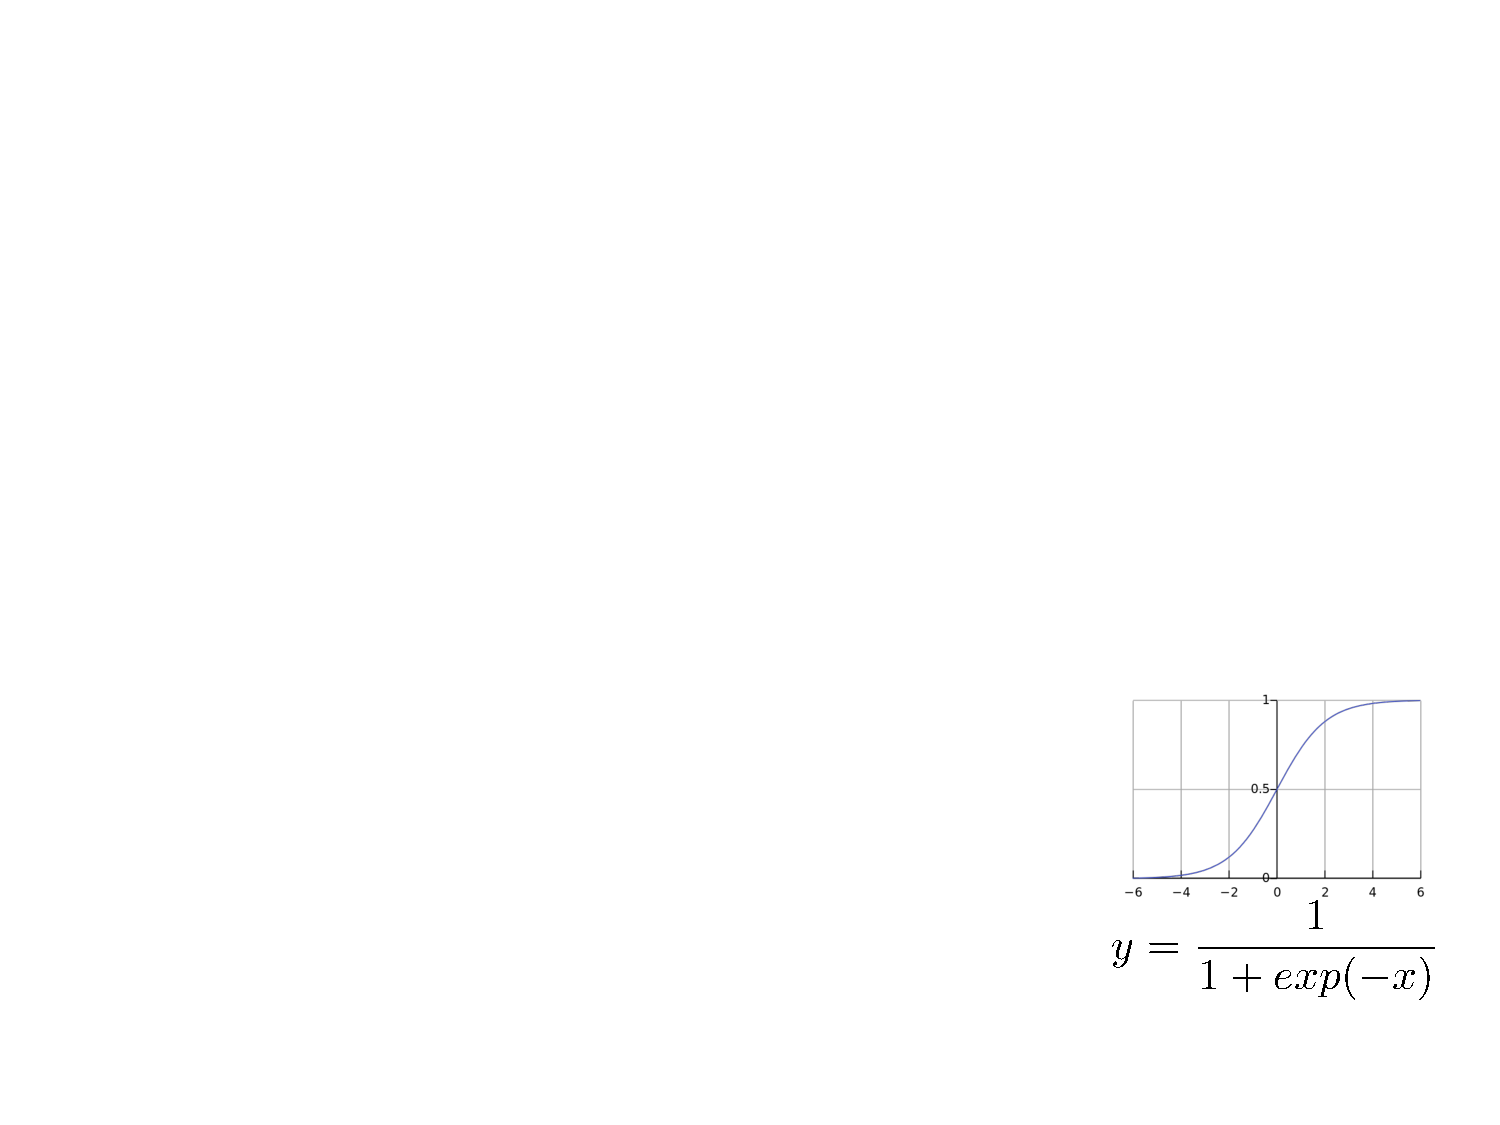
\includegraphics[width=1in]{figures/logistic.pdf}     \hfill \\
 \hfill \\
 
Making a decision boundary out of logistic equations:  \hfill \\
Output the $Y$ with the highest $P(Y|X)$.   \hfill \\
If binary Y, output Y=1 if $\displaystyle 1 < \frac{P(Y=1|X)}{P(Y=0|X)}$  \hfill \\
That simplifies to just $1 <exp(w_0 + \sum_i w_i X_i)$ or \hfill \\
$0 <w_0 + \sum_i w_i X_i$   \hfill \\
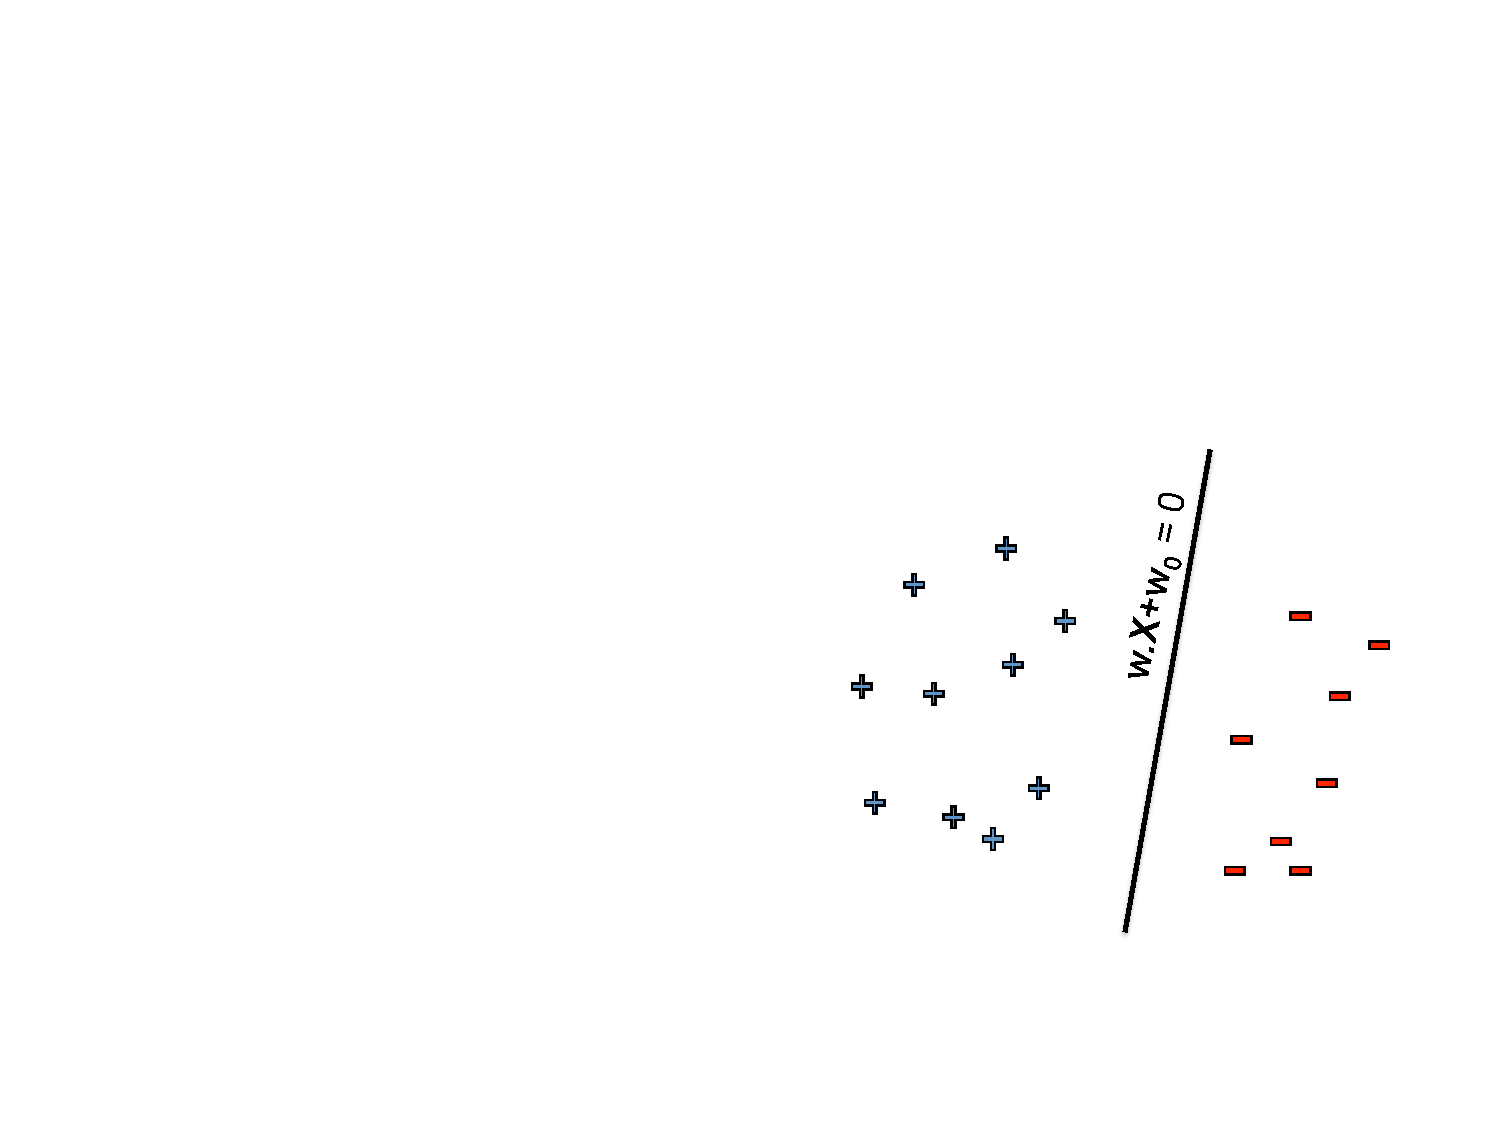
\includegraphics[width=.8in]{figures/logistic_boundary_linear.pdf}     \hfill \\
\textbf{The decision boundary is a line (or hyperplane), hence we have a linear classifier!} \hfill \\  \hfill \\

For $ \displaystyle P(Y=0 | \bm{X,w}) = \frac{1}{1 + exp(w_o + w_1 x_1)}$:  \hfill \\
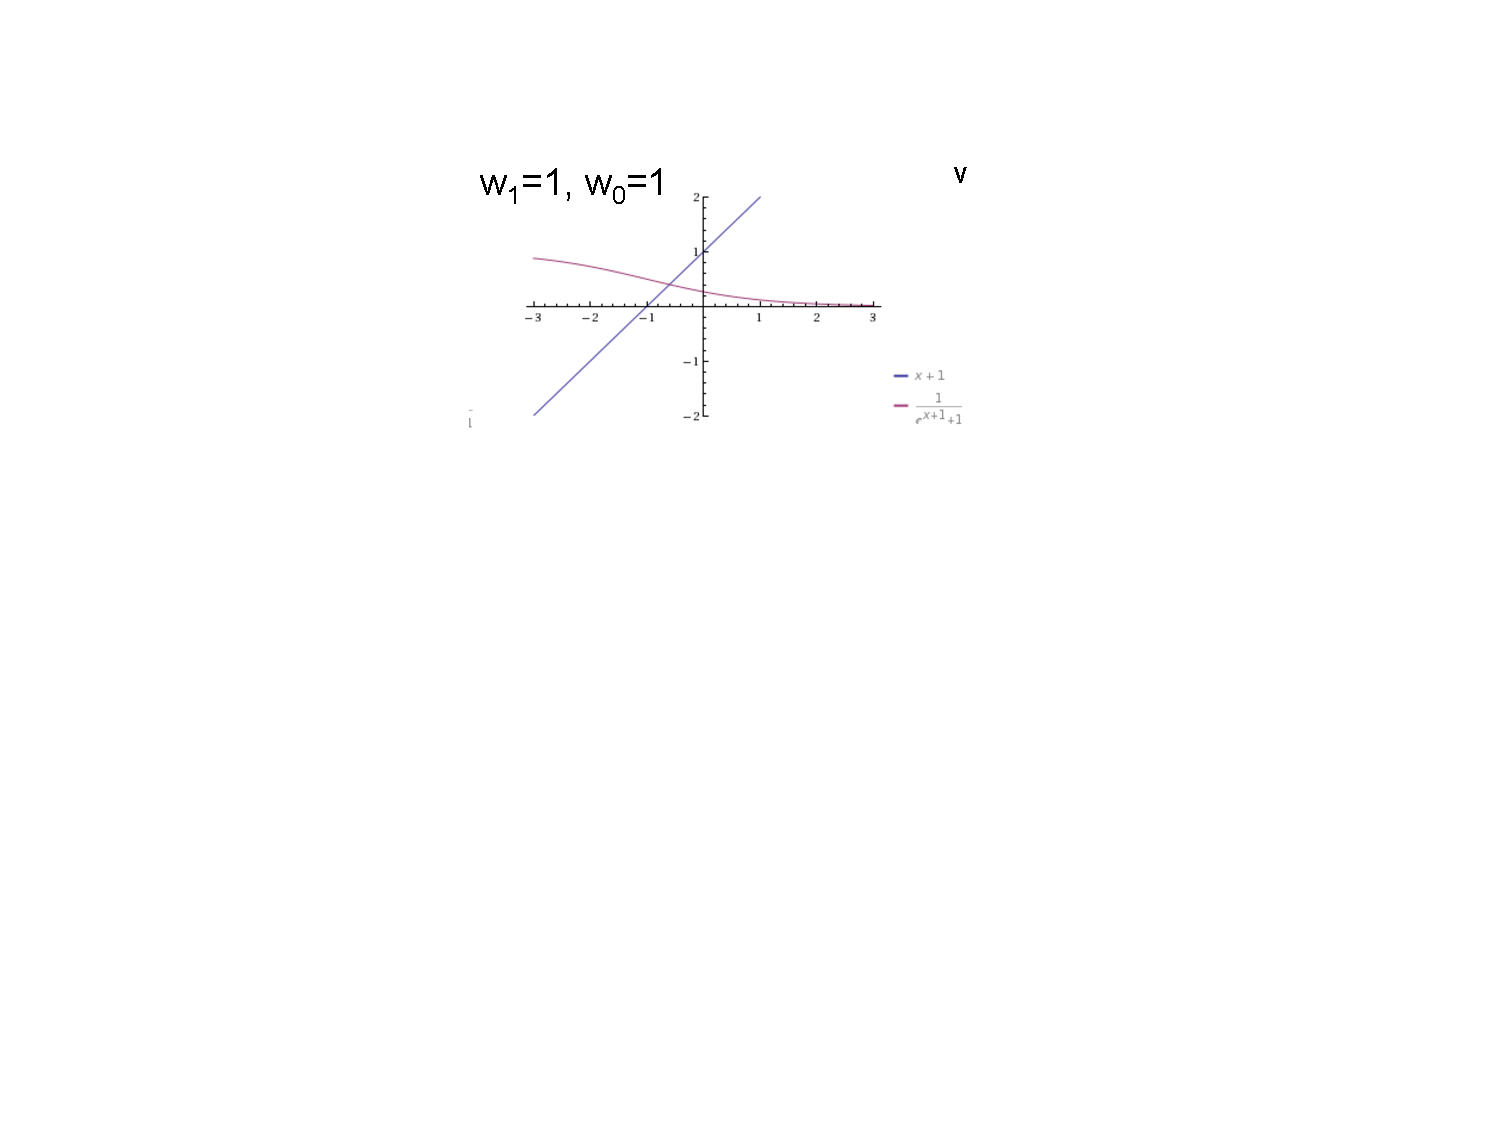
\includegraphics[width=2in]{figures/decision_boundary_example.pdf}   \hfill \\
(See notes for more $w_0, w_1$ values plotted.)  \hfill \\
In these plots, Y is the probability that the class is 1.    \hfill \\
The red curve is the sigmoid.  The blue line is the decision boundary.  \hfill \\
The decision boundary is from the equation $0 = w_1X + w_0$.  \hfill \\
% Erick advice: ignore the blue lines entirely.  don't need them to find probability distribution. 

\hfill \\
Larger weights result in a sharper curve.  The bias $w_0$ shifts there the middle of the curve is.   \hfill \\
The red sigmoid defines a probability distribution over $Y$ in \{0,1\} for every possible input X. \hfill \\
\hfill \\
The decision boundary leads to $P(Y=0|X, w) = 0.5$ when you are at the $y=0$ point on the line.   \hfill \\
(E/J words:  when the blue line crosses the x axis, that's when the sigmoid curve is above 1/2, which corresponds to classifying it as a no/0.)  \hfill \\
The slope of the line defines how quickly the probabilities go to 0 or 1 around the decision boundary. 
\hfill \\

2D inputs: \hfill \\
For $ \displaystyle P(Y=0 | \bm{X,w}) = \frac{1}{1 + exp(w_o + w_1 x_1 + w_2 x_2)}$:  \hfill \\
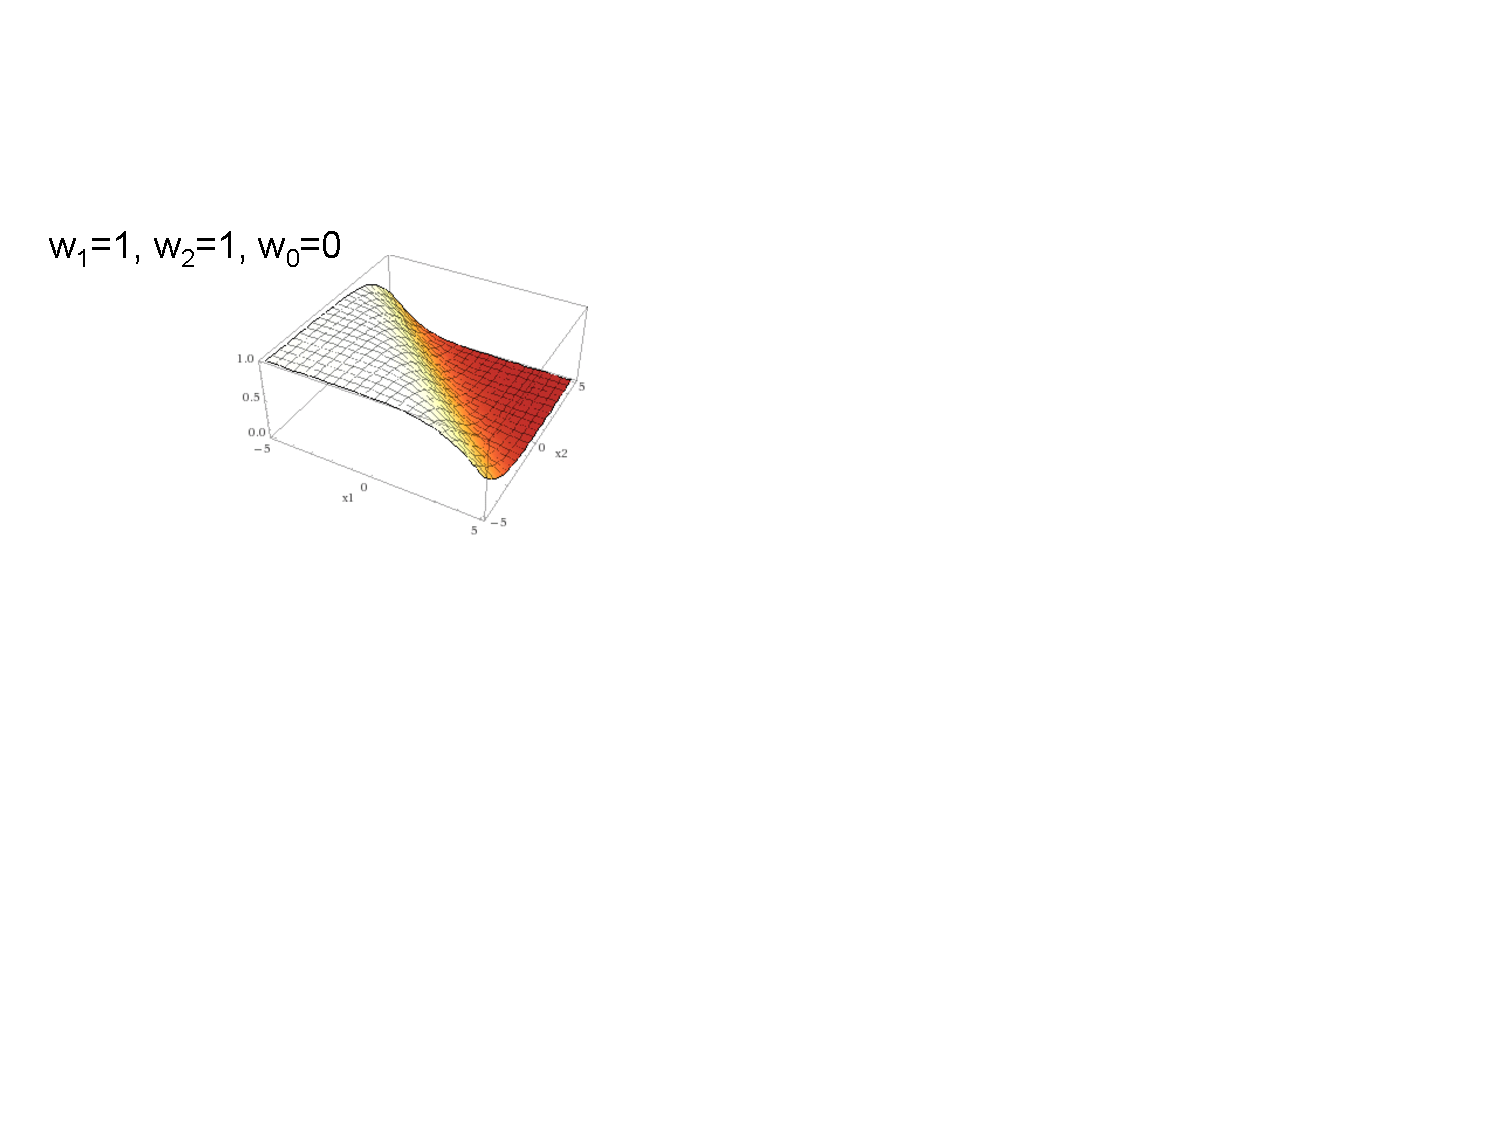
\includegraphics[width=2in]{figures/decision_boundary_example-2D.pdf}   \hfill \\

$P(Y=0 | X, w)$ decreases as $w_0 + \sum_i w_i x_i$ increases. 
Again, if you set the stuff inside the exponential to zero, you get the decision boundary hyperplane.

\subsubsection{Finding the w coefficients}
Generative (Naive Bayes) loss function: 
Now $j$ is a data point with observations indexed over $i$.


\begin{align*}
	\ln P(D | \bm{w}) = \sum_{j=1}^N  &  \ln P(x^j, y^j | \bm{w}) \mbox{   } \mbox{    (the full log-likelihood)}\\
					& \mbox{use Bayes' rule to rewrite conditionally}  \\  % J added this line. 
					= \sum_{j=1}^N  &  \ln [P(y^j | x^j, \bm{w}) P(x^j | \bm{w})] \\ % J added this line. 
				=  \sum_{j=1}^N  & \ln P(y^j | x^j , \bm{w}) + \sum_{j=1}^N \ln P(x^j | \bm{w})
\end{align*}

We decide to ignore the 2nd term because it won't help you get better predictions for that data anyway. 
Or, "From a machine learning perspective, "God gave us the data" and we don't care about the 2nd sum."  % Erick 2/6/2016

Professor Farhadi is calling this first time a discriminative (logistic regression) loss function:  \hfill \\
It is helping you discriminate between different classes.  It's not going to help you model the data. 
This is unlike regression; we don't care about the value it puts out.  We only care about what the resulting class is.  \hfill \\

% Erick. 
This is the difference between statistics and machine learning.  We only care about getting the best $\bm{w}$ for discriminating between classes. 

\textbf{Conditional Data Likelihood:} 
"Conditional" because you are conditioning on what $\bm{X}$ is. 
\begin{align*}
	\ln P(D_Y | D_{\bm{X}}, \bm{w}) = \sum_{j=1}^N \ln P(y^j | \bm{x}^j, \bm{w})
\end{align*}
$D_Y$ = ???  \hfill \\
$D_{\bm{X}}$ = ???   \hfill \\
Doesn't waste effort learning $P(X)$.  Focuses on $P(Y| \bf{X})$, which is all that matters for classification. \hfill \\
Discriminative models cann't compute $P(\bm{x}^j | \bm{w})$!  ??? 
\hfill \\

\subsubsection{Conditional Log Likelihood}
Just need to figure out how to go up and find the maximum likelihood. 

(the binary case only).  \hfill \\
$P(Y=0 | \bm{X}, \bm{w}) = \frac{1}{1 + \exp(w_0 + \sum_i w_i X_i)}$  \hfill \\
$P(Y=1 | \bm{X}, \bm{w}) = \frac{\exp(w_0 + \sum_i w_i X_i)}{1 + \exp(w_0 + \sum_i w_i X_i)}$  \hfill \\

($ l( \bm{w} )$ is conditional data log-likelihood.)  
\begin{align*}
	l( \bm{w})  \equiv  &  \sum_j \ln P(y^j | x^j, \bm{w})  \\
	& \mbox{Since $y^j$ is in \{0, 1\}, sum over the two cases: }   \\
	& \mbox{(the $y^j$ and $(1-y^j)$ act like delta functions)}   \\
	l(\bm{w})  =  & \sum_j y^j \ln P(y^j = 1 | x^j, \bm{w}) +(1 - y^j) \ln P(y^j = 0 | x^j, \bm{w})  \\
	& \mbox{plug in the definition of the likelihoods and do algebra to get:}  \\
	=& \sum_j  y^j (w_0 + \sum_i^n w_i x_i^j)  - \ln(1 + \exp(w_0 + \sum_i^n w_i x_i^j)) 
\end{align*}	

While we can't find a closed-form solution to optimize $l(\bm{w})$,  $l(\bm{w})$ is concave so we can to gradient \underline{as}cent. 
Jsut need to figure out how to go up and find the maximum likelihood.   % Wk 5 audio

\subsubsection{Gradent ascent to optimize w}
To maximize, we can't take derivative w.r.t $\bm{w}$ and optimize b/c no closed form solution.  % Wk 5 audio 
Instead we form the gradient vector and move along the gradient. % Wk 5 audio
Conditional likelihood for Logistic Regression is convex.  (see above)  \hfill \\
In this case it doesn't matter b/c we have a concave function.  % Wk 5 audio
Iterate to find $\bm{w}$: start somewhere, find gradient direction, make step in that direction, repeat, repeat.
\hfill \\

\textbf{Gradient}:  gives ascent or descent direction. \hfill \\
\begin{align*}
	\nabla_w l(\bm{w}) = [\frac{\partial l(\bm{w})}{\partial w_0}, \dots, \frac{\partial l(\bm{w})}{\partial w_n}]'  \hfill \\
\end{align*}
	(The $'$ at the end is for transpose b/c usually a column vector.)  \hfill \\
\textbf{Update Rule:} \hfill \\
\begin{align*}
	\Delta \bm{w} &= \eta \nabla_{\bm{w}} l(\bm{w})
\end{align*}
$\eta$ is the learning rate.  $\eta > 0$.  
	It can't be too big or you can get lost.  
	It can't be too small or you take forever to converge. 

Your next weights $(t+1)$ become: 
$w_i^{(t+1)} \leftarrow w_i^{(t)} + \eta \frac{\partial l(\bm{w})}{\partial w_i}$   \hfill \\
\hfill \\
Gradient ascent is the simplest  of optimization approaches.  
Note that conjugate gradient ascent is much better (see reading).(?)  \hfill \\

See slides for derivation of: \hfill \\
$\displaystyle \frac{\partial l(w)}{\partial w_i} = \sum_j x_i^j (y^j - P(Y^j = 1 | x^j, w))$

\subsubsection{Example of gradient ascent to maximize conditional log likelihood}
(M(C)LE; C for conditional) \hfill
Learning an approximation of the step function.  % Wk 5 audio. 

Use the equations: \hfill \\
\begin{itemize}
	\item \textbf{eq 1:} $w_i^{(t+1)} \leftarrow w_i^{(t)} + \eta \frac{\partial l(\bm{w})}{\partial w_i}$
	\item \textbf{eq 2:} $\displaystyle \frac{\partial l(w)}{\partial w_i} = \sum_j x_i^j (y^j - P(Y^j = 1 | x^j, w))$
			 The loss function is conditional on log likelihood.  % Wk 5 audio
	\item \textbf{eq 3:} $P(Y=1 | X, W) = \frac{\exp(w_0 + \sum_i w_i X_i)}{1 + \exp(w_0 + \sum_i w_i X_i)}$
	\item \textit{note:} superscript is for the $j^{th}$ data point and 
			subscripts are for the $i^{th}$ value of the input ($x$) array.  
			Don't forget that there is an $i=0$ $(x_0 = 1)$ bias term. 
\end{itemize}
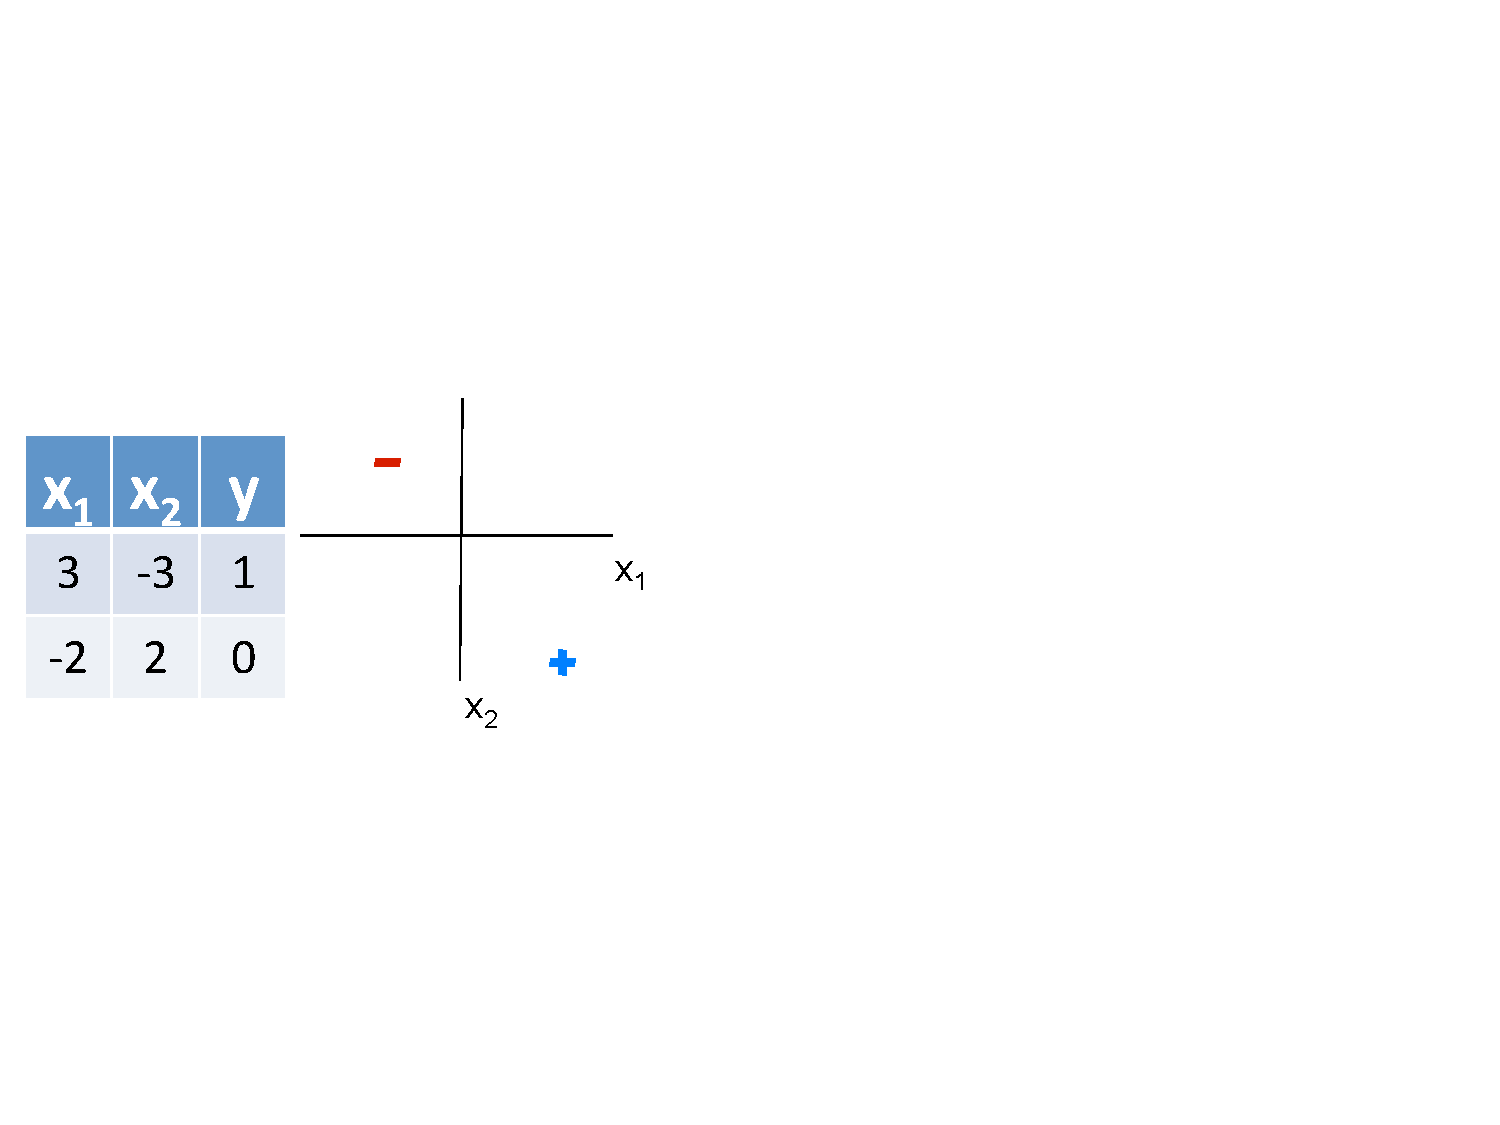
\includegraphics[width=1.5in]{figures/gradient_ascent_logistic_regression.pdf}   \hfill \\
\begin{itemize}
	\item begin with t=0 and $w = [w_0 + w_1 + w_2] = [0, 0, 0]$
	\item calculate \textbf{eq 3} for each Y.  
		\begin{itemize}
			\item For j = 0:  
				\begin{align*}
					P(Y^0 = 1 | x^0, w) &= \frac{\exp(0 + 0*3 + 0^(-3))}{(1 +  \exp(0 + 0*3 + 0*(-3)))} \\
						&= 1/(1+1) = 1/2
				\end{align*}
			\item For j = 1:  
				\begin{align*}
					P(Y^1 = 1 | x^1, w) &= \frac{\exp(0 + 0*(-2) + 0^(2))}{(1 +  \exp(0 +  0*(-2) + 0^(2)))} \\
						&= 1/(1+1) = 1/2
				\end{align*}
		\end{itemize} 
	\item calculate the terms that go into \textbf{eq 2} by looping over the 3 values of $i$ (bias and two other coefficients) and 2 values of $j$ (2 data points).  
		\begin{itemize}
			\item for $i=0, j=0$: ($j=$0th (1st) training example, bias term) \hfill \\
				 $x_0^0(y^0 - P(Y^0=1|x^0, w)) = 1(1-0.5) = 0.5$ 
			\item for $i=0, j=1$: ($j=$1st (2nd) training example, bias term) \hfill \\
				 $x_0^0(y^0 - P(Y^0=1|x^0, w)) = 1(0-0.5) = -0.5$ 
			
			\item for $1=1, j=0$: ($j=$0th (1st) training example, $x_1$ term) \hfill \\
				 $x_1^0(y^0 - P(Y^0=1|x^0, w)) = -2(1-0.5) = 1.5$ 
			\item for $i=1, j=1$: ($j=$1st (2nd) training example, $x_1$ term) \hfill \\
				 $x_1^1(y^1 - P(Y^1=1|x^1, w)) = -2(0-0.5) = 1.0$ 
				 
			\item for $1=2, j=0$: ($j=$0th (1st) training example, $x_2$ term) \hfill \\
				 $x_2^0(y^0 - P(Y^0=1|x^0, w)) = -3(1-0.5) = -1.5$ 
			\item for $i=2, j=1$: ($j=$1st (2nd) training example, $x_2$ term) \hfill \\
				 $x_2^1(y^1 - P(Y^1=1|x^1, w)) = 2(0-0.5) = -1.0$ 
		\end{itemize}
	\item Now we can compute the gradient (\textbf{eq 2}):
		\begin{itemize}
			\item $\nabla_w l(\bm{w}) = [\frac{\partial l(w)}{\partial w_1}, \frac{\partial l(w)}{\partial w_2}, \frac{\partial l(w)}{\partial w_3}]$
				\begin{align*}
					%\frac{\partial l(w)}{\partial w_i} &= \sum_j x_i^j (y^j - P(Y^j = 1 | x^j, w)) \\
						&= [0.5 - 0.5, 1.5 + 1.0, -1.5 - 1] = [0, 2.5, -2.5]
				\end{align*}
		\end{itemize}
	
	\item Use $\eta = 0.1$ to scale the gradient:  (\textbf{eq 1}) \hfill \\
			$w = [0,0,0] + 0.1*[0, 2.5, 2.5] = [0, 0.25, -0.25]$
	\item Start over with \textbf{eq 3} and updated $w$.
		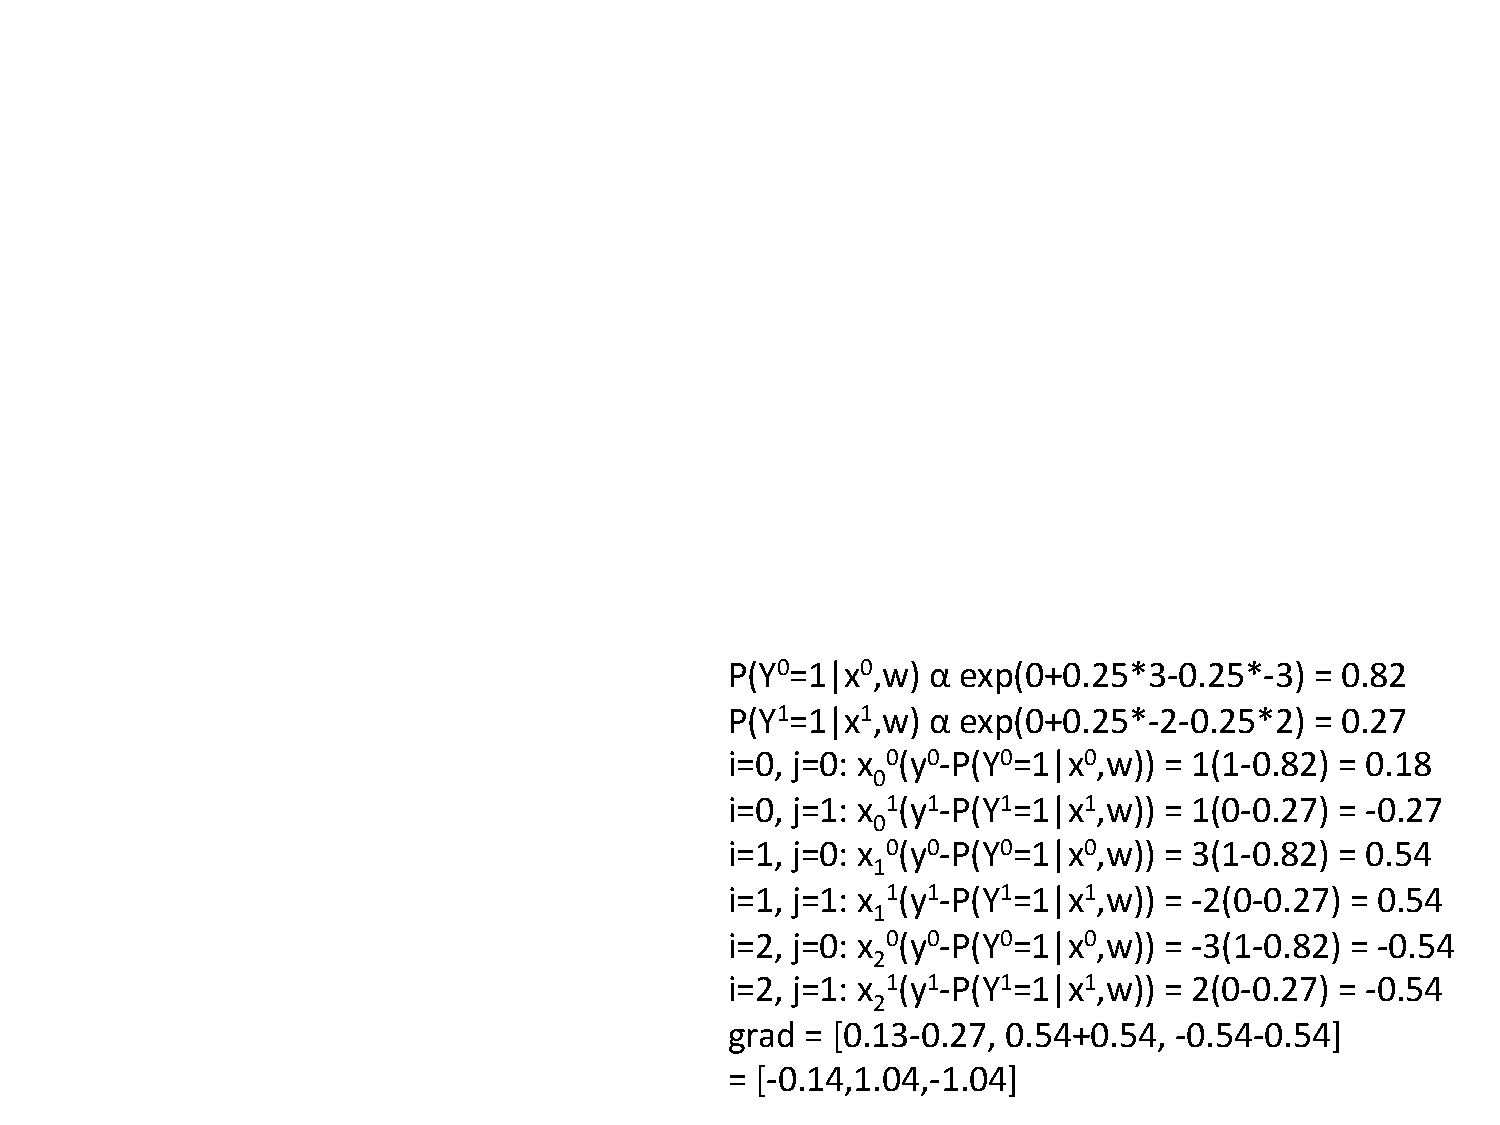
\includegraphics[width=2in]{figures/logistic_regression_ex_loop_2.pdf}
\end{itemize}

How to do more algorithmically:  \hfill \\
You don't have to get all the info to update all the weights at once.  
Do them one at a time.  \hfill \\
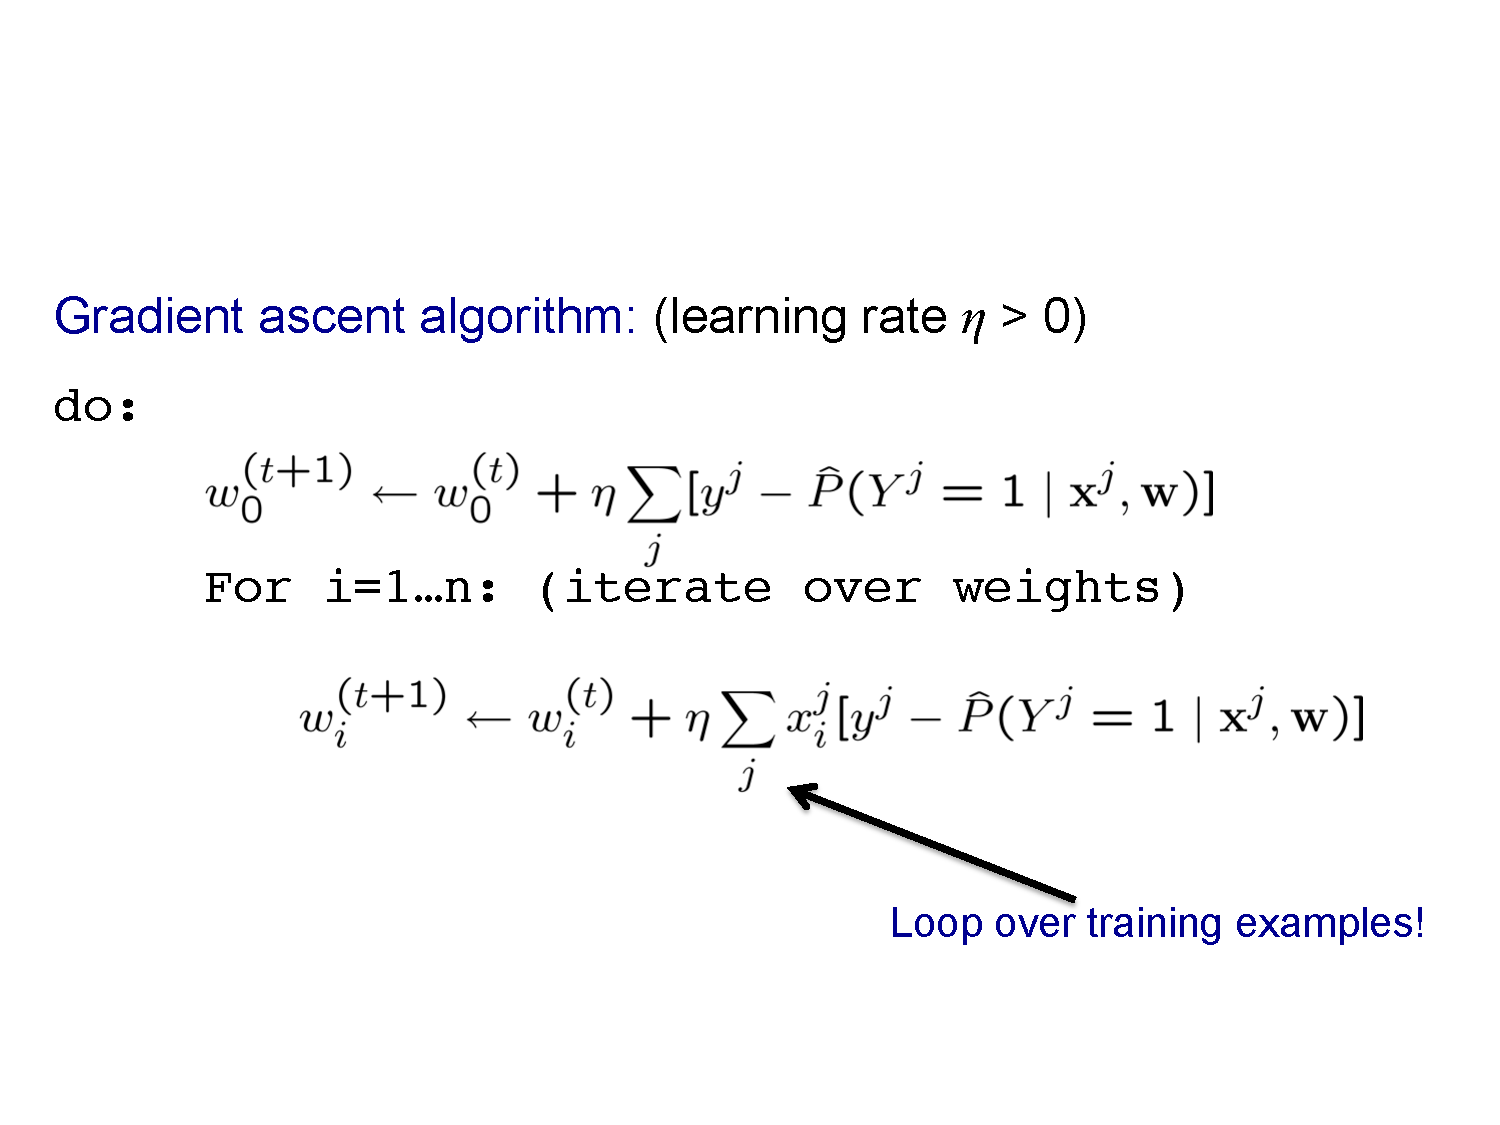
\includegraphics[width=2.5in]{figures/gradient_descent_algorthim.pdf}

\underline{How do you decide when to stop?} \hfill \\
(Not in notes!) \hfill \\

You need a criteria that tells you when to stop updating your gradient. 
	Use a threshold for magnitude of the gradient. 
	When the amount of change is small it is not changing a lot.  If concave, you are close to global optima. 

Why don't we wait until it gets to zero? 
	The chances of us hitting zero is low, and we might spend a lot of time wasting CPU cycles on negligible changes. 
	
When we are really far from the global optimum we can afford to take bigger steps. 
	Think about the objective function.  We can afford to make big steps if we are far.  
	If we make big steps when close, we can get farther away .

You could use this policy: let $\nu$ be big at the beginning of a loop counter. 
	Increase the value until you see a drop.
	"Line search" asks "what is maximum value of this parameter that gives you no drop?"  


\subsubsection{Overfitting in Logistic Regression}
 
 \underline{Intro \#1:}  \hfill \\
Be weary of large parameters.  % Audio wk 5
	Large parameters (large $a$ in $\frac{1}{1 + \exp(-a)}$) lead to a step function.  
	That's ok if you truly want a step, but you should be concerned about overfitting the minute you see a large parameter.
	We could regularize again: apply a penalty for large parameters. 
    	Could do something like maximizing $w^* = \argmax_w l(w) - \lambda*(||w||_2^2)$ instead of $w* =  \argmax_w l(w)$. 
	But that's not ideal.  Might have a hard time finding a suitable value for $\lambda$.  \hfill \\
	
	
Instead, use a probabilistic way of regularization.
	We've done this before using a prior.  
	Instead of MLE, we did MAP. The prior regularizes. 
	$P(w | Y, X) \propto P(Y | X,w)P(w)$.
	What would be the form of our prior ($P(w)$) be? 
	We want the posterior to be differentiable.  
	The likelihood was a sigmoid shape, so the log likelihood had the form of was of the form $e^{something}$.
	We already  know how to get the conditional likelihood in the form of $e^{blah}$.
	Well behaved summation of terms.   \hfill \\

We pick a gaussian distribution for the prior for mathematical convenience.
	We wanted to form a function we can optimize.
	If it doesn't come from gaussian and does come from multinomial, what happens? 
	We wouldn't be too wrong.  And it is just a regularization.  
	We are just trying to constrain $\bm{w}$ with something that is mathematically well behaved.
	Usually the prior is off. But it is only there to keep w from getting too big.  It gives a low score when w is too big.   \hfill \\

Q from student: why aren't we considering $P(X,W)$ as the prior? Why $P(Y|X, w)$?
	P(X,W) is discriminative.  
	We aren't reformulating our problem.  Just looking to estimate the parameters. 
	We want to regularize the parameter not the data (?).    \hfill \\
 
 \underline{Intro \#2:}   \hfill \\
 
Like in linear regression, the maximum likelihood solution prefers higher weights.  
Higher weights can give higher likelihood of properly classifying examples close to the decision boundary.  
This over-fitting causes features to have larger influences on the decision:  \textbf{beware of overfitting!!!}. 
Again, you can use regularization to penalize high weights.
This will be covered more later. 
\hfill \\

\subsubsection{MAP for Logistic Regression}
Above was M(Conditional)LE.     \hfill \\
Recall that the MAP/MLE difference is \_\_\_\_\_\_\_\_\_.  \hfill \\
Priors on $\bm{w}$ are commonly added for regularization.    \hfill \\
Helps avoid very large weights and overfitting.    \hfill \\
$P(\bm{w} | Y, \bm{X}) \propto P(Y | \bm{X}, \bm{w} ) P(\bm{w} )$  \hfill \\
Use a normal distribution with zero mean and "identity covariance".  (\_\_\_\_):  \hfill \\
$ \displaystyle  P(\bm{w} ) = \prod_i \frac{1}{\kappa \sqrt{2 \pi}} e^{\frac{-w_i^2}{2 \kappa^2}}$ \hfill \\
$\kappa^2$ is variance.  \hfill \\
\hfill \\

Now we form our MAP estimate: 
\begin{align*}
	w* &= \argmax_w \ln[P(\bm{w}) \prod_{j=1}^N P(y^j | x^j, \bm{w})]  \\
		&= \argmax_w \ln[ \prod_i \frac{1}{\kappa \sqrt{2 \pi}} e^{\frac{-w_i^2}{2 \kappa^2}}   \prod_{j=1}^N P(y^j | x^j, \bm{w})]
\end{align*}

 Instead of focusing on the stuff after the $\prod$ in the bracket we also have $P(w)$.
 Our prior, $P(w)$ is $\prod$ fo gaussians.
 The $\prod(y^j|x^, x_j)$ is called likelihood (???)  

Add $\log P(\bm{w})$ to the objective:
\begin{align*}
	\ln P(\bm{w}) & \propto - \frac{\lambda}{2} \sum_i w_i^2 \\
	\frac{\partial \ln P(\bm{w})}{\partial w_i} &= \lambda w_i
\end{align*}

We now have a new way of optimizing w.
This is a quadratic penalty (???) that drives the weights toward zero. \hfill \\
It adds a negative linear term to the gradients (???).  \hfill \\
Also applicable in linear regression! 

\subsubsection{Review: MLE vs. MAP for Logistic Regression}
\underline{Maximum conditional likelihood estimate:}
\begin{align*}
	w* &= \argmax_w \ln[\prod_{j=1}^N P(y^j | x^j, \bm{w})] \\
	w_i^{(t+1)} & \leftarrow w_i^{(t)} + \eta \sum_j x_i^j [y^j - \widehat{P}(Y^j = 1 | x^j, \bm{w})]\\
\end{align*}

\underline{Maximum conditional a posteriori estimate:}
\begin{align*}
	w* &= \argmax_w \ln[P(\bm{w}) \prod_{j=1}^N P(y^j | x^j, \bm{w})] \\
	w_i^{(t+1)} & \leftarrow w_i^{(t)} + \eta \{ -\lambda w_i^{(t)} +  \sum_j x_i^j [y^j - \widehat{P}(Y^j = 1 | x^j, \bm{w})]\\
\end{align*}
The $\lambda$ term complains when the value is big.
This $-\lambda$ if from the derivative of the gaussian.
The whole point: if you add a prior and take a derivative, it is a form of regularization and should act as a penalty on big $w$. 


\hfill \\  \hfill \\


Vocab \hfill \\
\begin{itemize}
	\item \textbf{discriminative}:  estimates joint probabilities.  E.g. $p(Data, Zebra)$, $p(Data, No Zebra)$. 
	\item \textbf{generative}:  E.g. $p(Zebra | Data)$, $p(No Zebra | Data)$. 
\end{itemize}

\subsubsection{Multiclass Logistic Regression (discrete labels)}
Define a weight vector $w_i$ for each $y_i$ where i ranges from $1$ to $R-1$ for $R$ classes.
You don't need a weight vector for the $R^{th}$ class b/c its probability is 1 - the sum of the rest.  \hfill \\
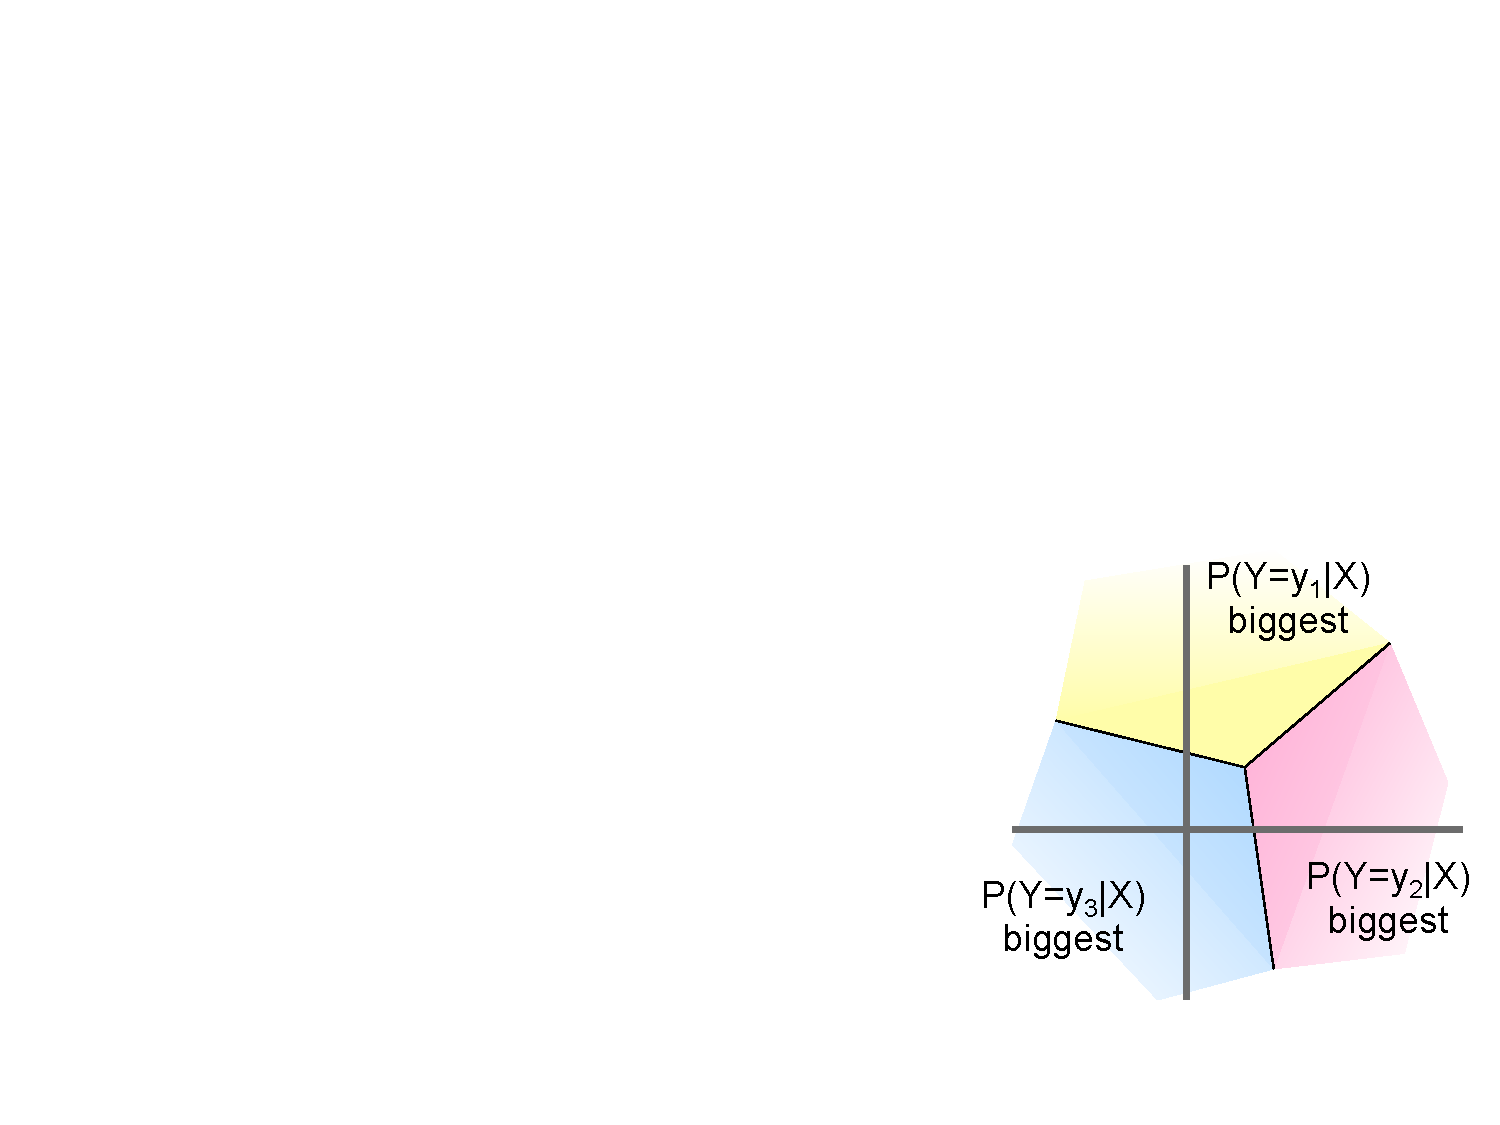
\includegraphics[width=1in]{figures/multiclass_logistic.pdf} \hfill \\
Each category will have its own w values.  \hfill \\ % Wk 5 audio. 
Don't need to train k w values.  k-1.  b/c they have to sum to 1.    % Wk 5 audio. 

\begin {align*}
	P(Y=1 | X ) & \propto \exp(w_{10} + \sum_i w_{1i}X_i)  \\
		& \mbox{note: $\bm{w}$ is now a matrix, not an array.}  \\
	P(Y=2 | X ) & \propto \exp(w_{20} + \sum_i w_{2i}X_i)  \\
	 & \dots \\
	 & \mbox{the last probability is defined relative to the rest.}  \\
	P(Y=r | X ) &= 1- \sum_{j=1}^{r-1} P(Y=j | X)
\end{align*}
After normalizing, your probabilities become: 
\begin {align*}
	P(Y=y_k | X ) &=  \frac{\exp(w_{k0} + \sum_{i=1}^n w_{ki} X_i)}{1 + \sum_{j=1}^{R-1} \exp(w_{j0} + \sum_{i=1}^n w_{ji}X_i)} \\
	& \mbox{the last class is 1 - the sum of the other probabilities:} \\
	P(Y=y_R | X ) &=  \frac{1}{1 + \sum_{j=1}^{R-1} \exp(w_{j0} + \sum_{i=1}^n w_{ji}X_i)} 
\end{align*}
Note: features can be discrete or discontinuous. 

\subsubsection{Gaussian Naive Bayes vs Logistic Regression.}
Gaussian Naive Bayes with class-independent variances is representationally equivalent to Linear Regression.
("If you do have an infinite number of training examples, the GNB and LR produce identical classifiers.")  % Erick 2/7
The solutions different because of the objective (loss) function.  \hfill \\

If you do have class-independent variances and the underlying model is gaussian, GNB does better than LR.
You get an incorrect model for GNB if you don't have class-independent variances.  %Erick
LR is less biased because it does not assume conditional independence.  % Erick.
 \hfill \\  \hfill \\

You could use either to learn $ f: X \rightarrow Y$ for $X$ that is a vector of real-valued features ($< X_1, \dots, X_n >$) and boolean Y. \hfill \\ \hfill \\

The two approaches make different assumptions:   \hfill \\
\begin{itemize}
	\item NB assumes features are independent given the class.  This is an assumption on $P(\bm{X} | Y)$.
	\item LR assumes functional form of $P(Y|\bm{X})$, and makes no assumption on $P(\bm{X} | Y)$.
\end{itemize}

Gaussian Naive Bayes classifier would assume: \hfill \\
\begin{itemize}
	\item all $X_i$ are conditionally independent given Y.  
		If you fix what hump you are looking at, you don't need to worry about the rest of the parameters. 
	\item model $P(X_i | Y = y_k)$ as Gaussian with $N(\mu_{ik}, \sigma_i)$.  (Your inputs are each produced by a gaussian.)
	\item model $P(Y)$ as Bernoulli$(\theta, 1-\theta)$
\end{itemize} 
This implies the form of $P(Y|X)$ is:
$\displaystyle P(Y=1 | X= < X_1, \dots, X_n >) = \frac{1}{1 + \exp(w_0 + \sum_i w_i X_i)}$. \hfill \\
In the slides, he derives the form.   \hfill \\
(??)  You see that if you assume Gaussian in Logistic Regression, you get: \hfill \\
 $w_0 = \ln \frac{1 - \theta}{\theta} + \frac{\mu_{i0}^2 + \mu_{i1}^2}{2 \sigma_i^2}$ and $w_i = \frac{\mu_{i0} + \mu_{i1}}{\sigma_i^2}$
 
 His confusing summary: \hfill \\
 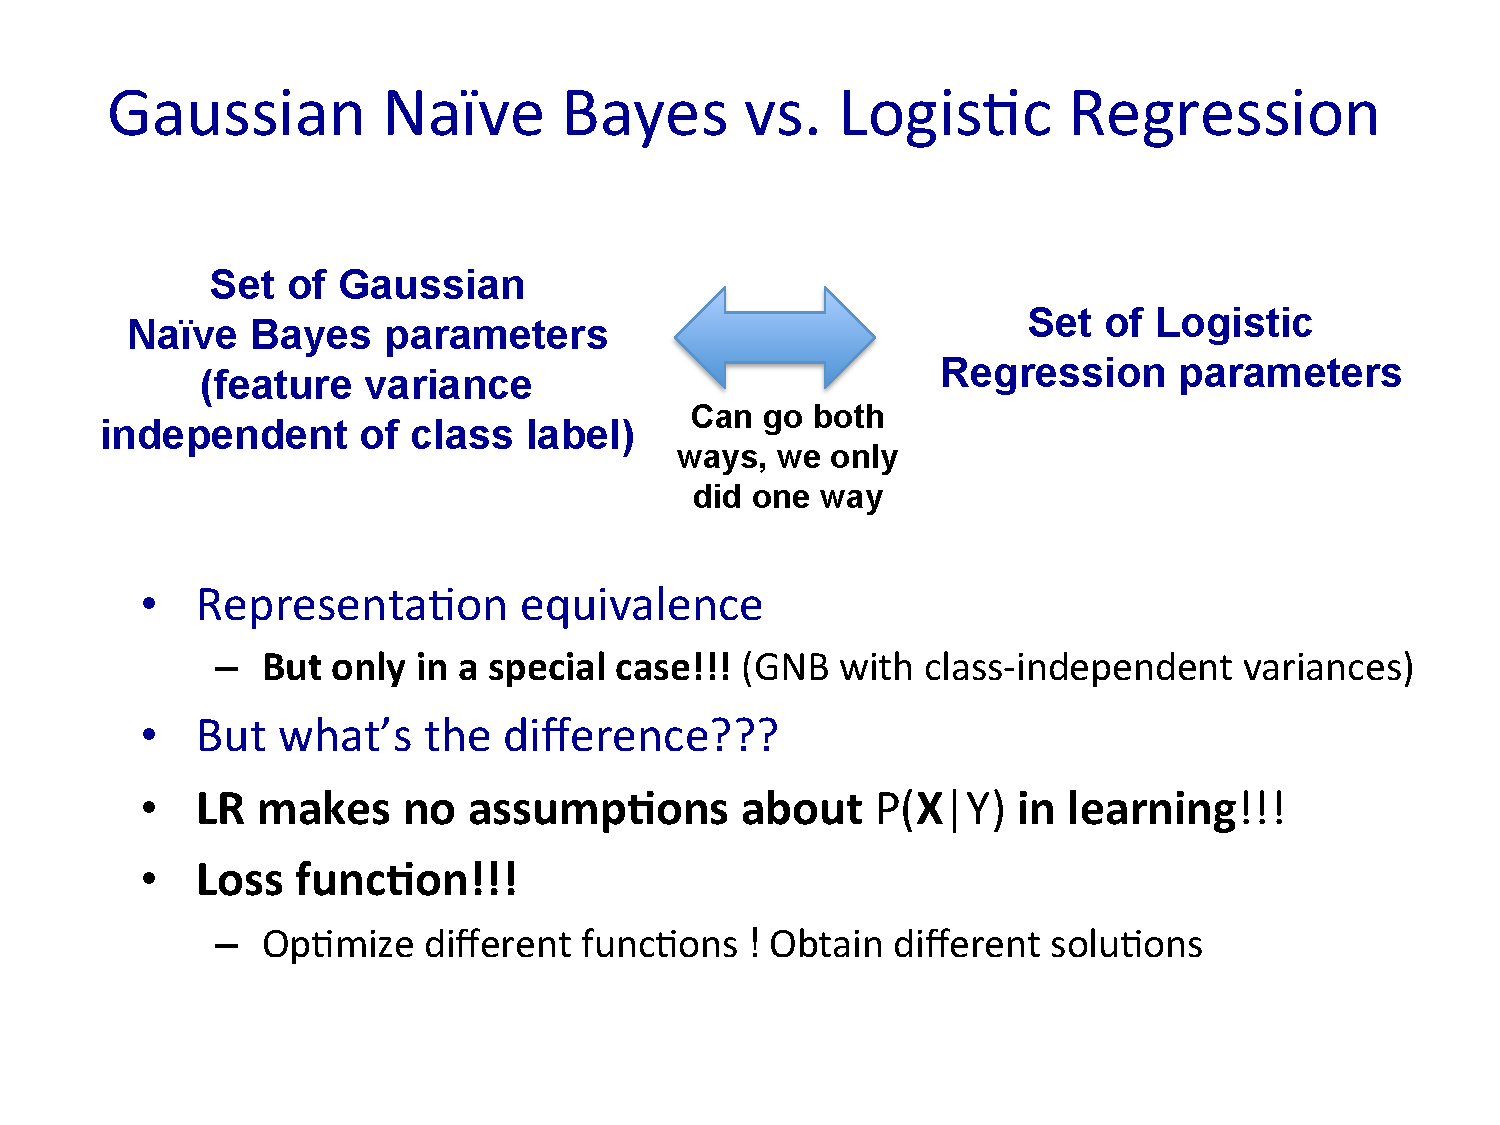
\includegraphics[width=2.5in]{figures/GNB_vs_LR.pdf}
 Attempted translation: 
 
 Note: you need more parameters to train Naive Bayes. \hfill \\
 $4n + 1$ parameters for GNB,  $n + 1$ parameters for Logistic Regression. \hfill \\
 The NB parameter estimates are uncoupled, so there are more of them.   \hfill \\
 (The Logistic Regression parameter estimates \underline{are} coupled.)

If you don't have infinite data (? "non-asymptotic analysis"): \hfill \\
For $n$ attributes in $X$, NB needs $O(\log n)$ samples to converge and Logistic Regression needs $O(n)$.  
So GNB converges more quickly to its (perhaps less helpful) "asymptotic estimates."

You have to do all of the optimization at once, all together if you are doing logistic regression.  ???
Easier in a certain sense to fit a Gaussian model. 
Typically we have a lot of data, and that data is not gaussian so Logistic Regression is probably better. 

\subsection{Logistic Regression Protocol}
Steps:
\begin{itemize}
	\item start with given data: x and labels.
	\item form conditional log likelihood function.
	\item either optimize that or add a prior
	\item do hill climbing until you stop seeing big changes in the weights
	\item then you claim victory
\end{itemize}

\textbf{For binary classification:} \hfill \\
The final output of trained regression is the weight vector, $w*$.
It is d+1 dimensional for a d-dimensional feature vector.  The +1 is for bias (that coefficient is 1).  \hfill \\

\underline{How do you use it?}  \hfill \\
You found the form of decision boundary was $P(Y=1|X,w) = exp()/(1+ exp())$.
Put in the $x$ with the $w$.  
Compute the probability of Y=0 and Y=1, pick the biggest result. 
How do you know if your weights are good? 
Test on held-out data (NOT the test data). 

\subsubsection{Andrew Ng}
* gives numbers between 0 and 1 (good for classification)   \hfill \\
* called "logistic regression" but it is really for classification.  (don't be confused by "regression") \hfill \\
* "sigmoid function" and "logistic function" are essentially synonymous.  \hfill \\
 
